\newgeometry{top=1cm, bottom=2cm}
\section{Methode der kleinsten Quadrate}
\begin{figure}[h!]
    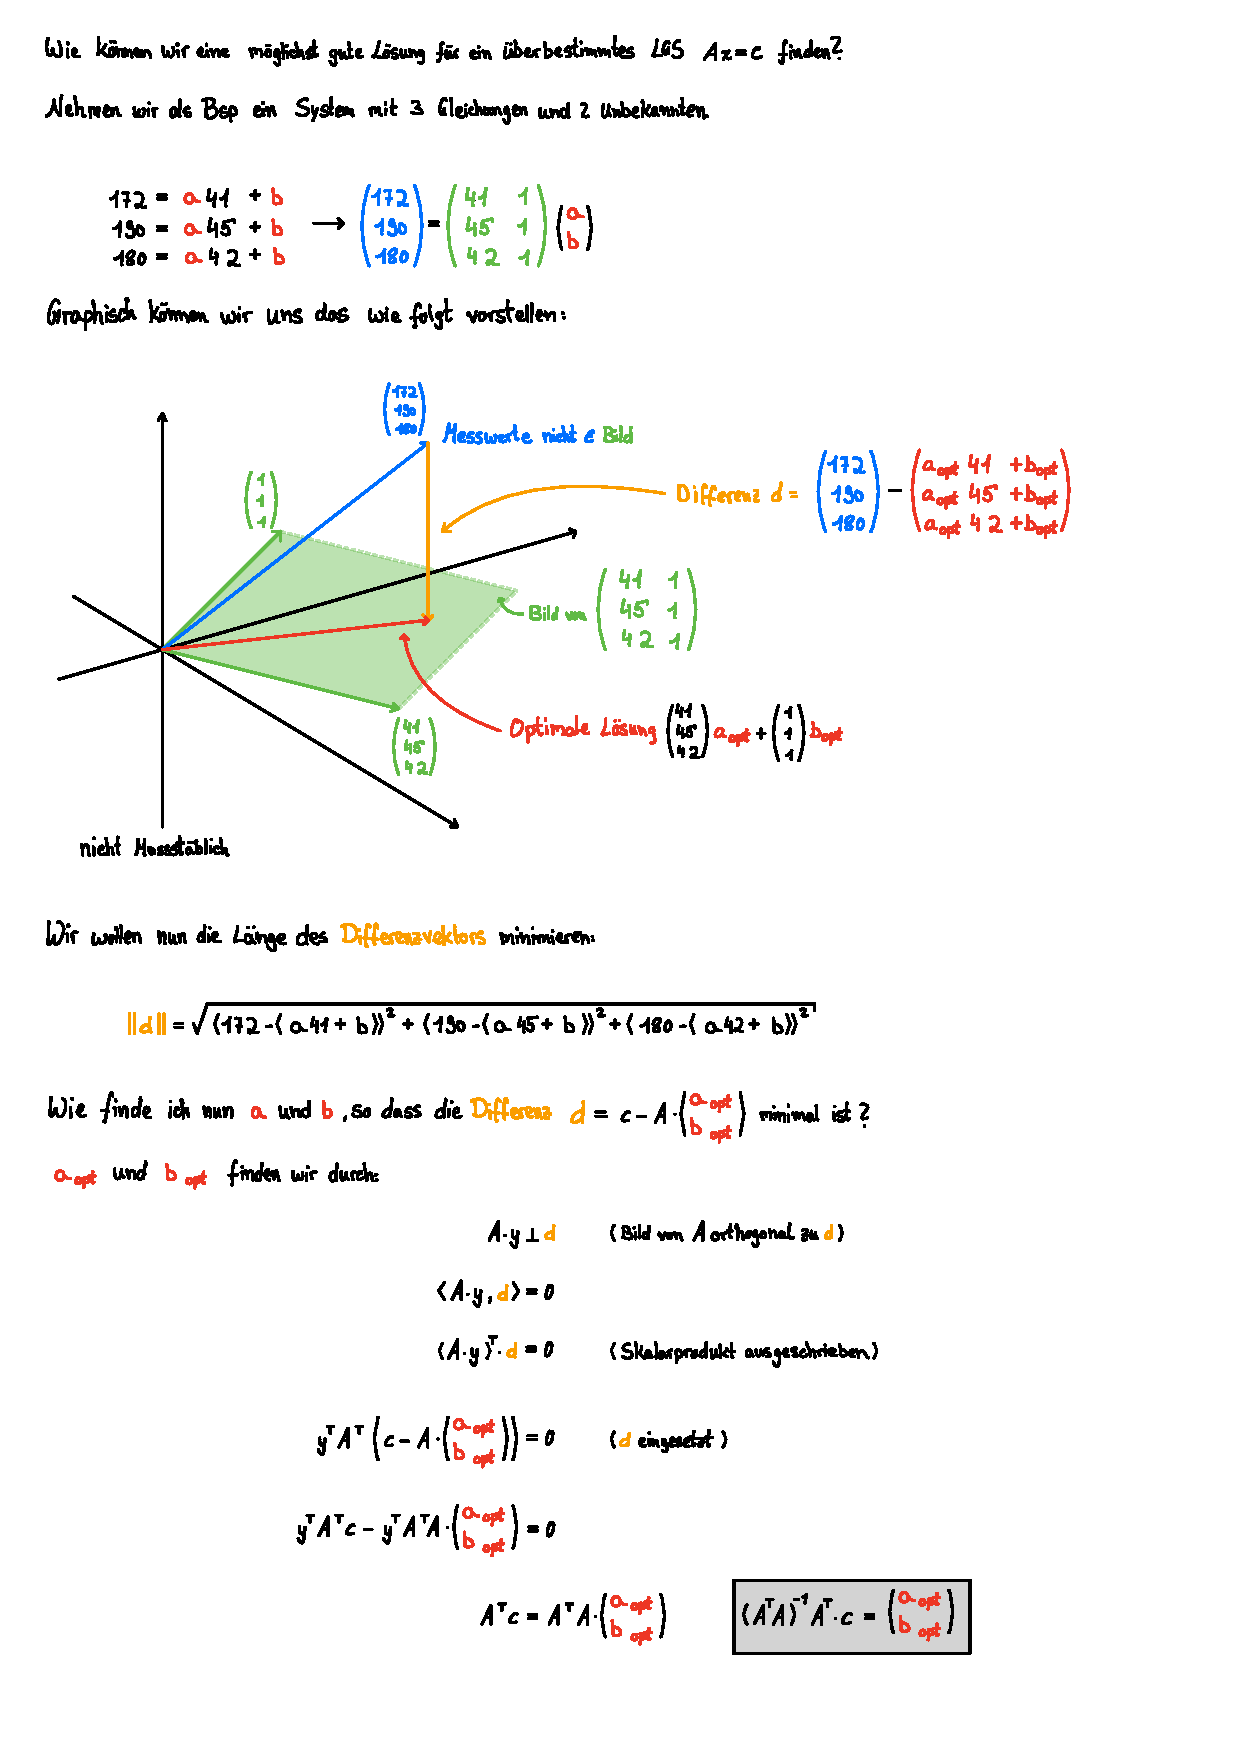
\includegraphics[page=1, scale=0.842]{pdf/07_Methode_der_kleinsten_Quarate.pdf}
\end{figure}
\newpage
\includepdf[pages={2-}, 
            pagecommand={\thispagestyle{plain}}, 
            scale=0.95]{pdf/07_Methode_der_kleinsten_Quarate.pdf}

\newgeometry{top=2.5cm, bottom=2cm}

\subsection{Beispielaufgaben} 

\vspace{1cm}

\subsubsection{} %Übung 09

Sei 

\begin{equation*}
    \begin{aligned}
        &x_1 +& 0&x_2 =& 2\\
        &x_1 +&  &x_2 =& 1\\
        &x_1 +& 2&x_2 =& 0\\
        &x_1 +& 3&x_2 =& -1\\
        &x_1 +& 4&x_2 =& 1 
    \end{aligned}
\end{equation*}

ein überbestimmtes lineares Gleichungssystem. Lösen Sie das Ausgleichproblem mittels der Methode der kleinsten Quadrate. Das heisst, finden Sie \( (\hat{x}_1,\hat{x}_2)^\top \), so dass \( \|r\|_2 = \|Ax-c\|_2 \) minimal ist.

\vspace{1\baselineskip}

\begin{solution}    

    \vspace{1\baselineskip}

    \leftskip=2em

    \begin{equation*}
        A = \begin{pmatrix}
            1 & 0\\
            1 & 1\\
            1 & 2\\
            1 & 3\\
            1 & 4
        \end{pmatrix}, \quad
        c = \begin{pmatrix}
            2\\
            1\\
            0\\
            -1\\
            1
        \end{pmatrix}
    \end{equation*}

    \vspace{1\baselineskip}

    \begin{equation*}
        A^\top A = \begin{pmatrix}
            1 & 1 & 1 & 1 & 1\\
            0 & 1 & 2 & 3 & 4
        \end{pmatrix} \begin{pmatrix}
            1 & 0\\
            1 & 1\\
            1 & 2\\
            1 & 3\\
            1 & 4
        \end{pmatrix} = \begin{pmatrix}
            5 & 10\\
            10 & 30
        \end{pmatrix}
    \end{equation*}

    \vspace{1\baselineskip}

    \begin{equation*}
        A^\top c = \begin{pmatrix}
            1 & 1 & 1 & 1 & 1\\
            0 & 1 & 2 & 3 & 4
        \end{pmatrix} \begin{pmatrix}
            2\\
            1\\
            0\\
            -1\\
            1
        \end{pmatrix} = \begin{pmatrix}
            3\\
            2
        \end{pmatrix}
    \end{equation*}

    Löse \( A^\top A \hat{x} = A^\top c \):

    \begin{equation*}
        \begin{gmatrix}[L]
            5 & 10 \\
            10 & 30
        \end{gmatrix} \hspace{-0.75em} \begin{gmatrix}[R]
            3 \\ 2
                \rowops
                    \add[-2]{0}{1}
        \end{gmatrix} \; \rightarrow \;
        \begin{gmatrix}[L]
            5 & 10 \\
            0 & 10
        \end{gmatrix} \hspace{-0.75em} \begin{gmatrix}[R]
            3 \\ -4
        \end{gmatrix} \; \rightarrow \; \left\{ \begin{aligned}
            \hat{x}_2 &= - \frac{2}{5} \\[0.5em]
            \hat{x}_1 &= \frac{7}{5}
        \end{aligned} \right.
    \end{equation*}
        

\end{solution}

\newpage

\subsubsection{}

Gegeben sei

\begin{equation*}
    \begin{aligned}
        &x_1 +&  &x_2 &- 1 =&\; r_1\\
        &     &  &x_2 &- 3 =&\; r_2\\
        &     &  &x_2 &- 4 =&\; r_3\\
    \end{aligned}
\end{equation*}

Lösen Sie das Ausgleichsproblem mittels der QR-Zerlegung. 

\vspace{1\baselineskip}

\begin{solution}    

    \vspace{1\baselineskip}

    \leftskip=2em

    \begin{equation*}
        A = \begin{pmatrix}
            1 & 1\\
            0 & 1\\
            0 & \textcolor{red}{1}
        \end{pmatrix}, \quad
        c = \begin{pmatrix}
            1\\
            3\\
            4
        \end{pmatrix}
    \end{equation*}

    \vspace{1\baselineskip}

    Das Element \( a_{32} \) muss eleminiert werden, wir notieren also
    
    \begin{equation*}
        i = 3, \ i = 2, \ a_{22} = 1, \ a_{32} = 1, \ \omega = \sqrt{2}. 
    \end{equation*}

    Dadurch ist

    \begin{equation*}
        Q^{\top} = \begin{pmatrix}
            1 & 0 & 0\\
            0 & \cos \varphi & \sin \varphi\\
            0 & -\sin \varphi & \cos \varphi
        \end{pmatrix} \ \text{mit} \; \left\{ \begin{aligned}
            \cos \varphi &= \frac{1}{\sqrt{2}}\\
            \sin \varphi &= \frac{1}{\sqrt{2}}
        \end{aligned} \right.
    \end{equation*}

    \vspace{1\baselineskip}

    \begin{equation*}
        Q^\top A = \begin{pmatrix}
            1 & 0 & 0\\
            0 & \cos \varphi & \sin \varphi\\
            0 & -\sin \varphi & \cos \varphi
        \end{pmatrix} \begin{pmatrix}
            1 & 1\\
            0 & 1\\
            0 & 1
        \end{pmatrix} = \begin{pmatrix}
            1 & 1\\
            0 & \sqrt{2}\\
            0 & 0
        \end{pmatrix} \; \rightarrow \; R_0 = \begin{pmatrix}
            1 & 1\\
            0 & \sqrt{2}
        \end{pmatrix}
    \end{equation*}

    \vspace{1\baselineskip}

    \begin{equation*}
        Q^\top c = \begin{pmatrix}
            1 & 0 & 0\\
            0 & \cos \varphi & \sin \varphi\\
            0 & -\sin \varphi & \cos \varphi
        \end{pmatrix} \begin{pmatrix}
            1\\
            3\\
            4
        \end{pmatrix} = \begin{pmatrix}
            1\\
            \frac{7 \sqrt{2}}{2}\\
            \frac{\sqrt{2}}{2}
        \end{pmatrix}  \; \rightarrow \; d_0 = \begin{pmatrix}
            1\\
            \frac{7 \sqrt{2}}{2}
        \end{pmatrix}
    \end{equation*}

    Nun lösen wir das Gleichungssystem \( R_0 \hat{x} = d_0 \):

    \begin{equation*}
        \begin{gmatrix}[L]
            1 & 1 \\
            0 & \sqrt{2}
        \end{gmatrix} \hspace{-0.75em} \begin{gmatrix}[R]
            1 \\ \frac{7\sqrt{2}}{2}
        \end{gmatrix} \; \rightarrow \; \hat{x} = \begin{pmatrix}
            -\frac{5}{2} \\
            \frac{7}{2}
        \end{pmatrix} 
    \end{equation*}

\end{solution}